\chapter{Prediction with Commit Data}
\label{chap:prediction}

% TODO discuss research question

% How the visualization helped 	
The visualization of the data collected about the projects help provide insights into data set. With the data visualized a more general look of the data collected is available. While creating the method for predicting change within the project the visualizations provided a helpful resource. The actual data used for training the prediction model is outlined in \autoref{sec:prediction_data}. After that the prediction model is detailed in \autoref{sec:prediction_method}. %Finally, the actual implementation is discussed in \autoref{sec:implementation}.

\section{Prediction Data}
\label{sec:prediction_data}

The data used for predicting changes with a project is originally from the visualizations. For more information about the specific information collected see  \autoref{sec:collection}, \autoref{sec:storage} and \autoref{sec:parsing}. More briefly, the commit data collected from the target \gls{oss} project is used to make predictions. The goal is to predict whether a method within a project will change within the next five commits. As outlined in \autoref{sec:parsing}, the different types of changes can be either additions, deletions, additions and deletions or no change at all.

The machine learning model requires samples from the data set to train from to allow for predictions of new elements. Also it is necessary for these samples to able to be categorized. This requirement provides some restrictions on which values can be included in the sampling. Since the categorization is methods that will change and those that will not change within the next 5 commits, data samples must know whether it will change or not within the next 5 commits. This therefore prevents data from the last 5 commits from being sampled for training the data model.

\begin{figure}[!ht]
    \centering
        %Generated from http://jsfiddle.net/5aubxshy/
        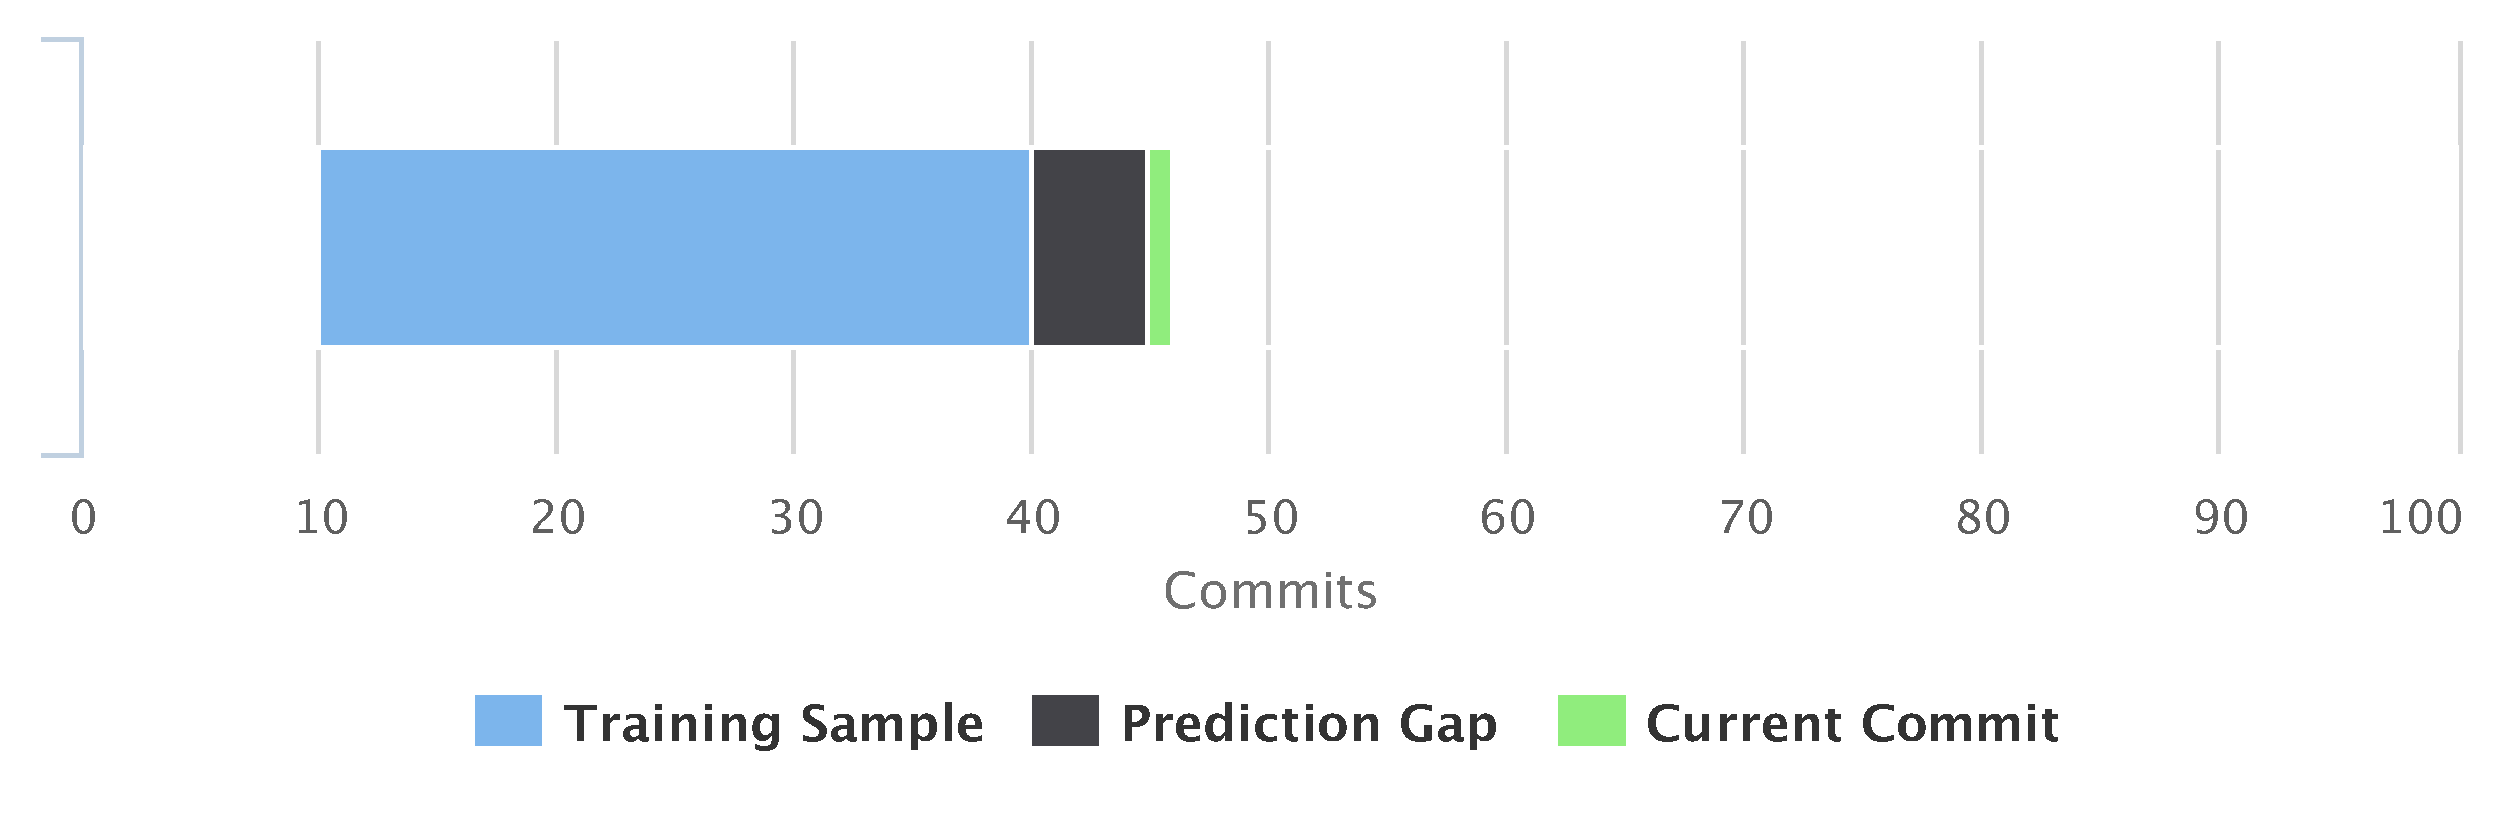
\includegraphics[width=1.0\textwidth]{images/training_sampling}
    \caption{Training Sampling Layout}
    \label{fig:training_data_range}
\end{figure}

The \gls{swr} is a second restriction placed on the sampling of data. The data will only be sampled within a limited range of commits as outlined in \autoref{fig:training_data_range}. In this case, the \gls{swr} is 30 and the gap is 5. The gap takes into account the first restriction, preventing sampling in the 5 latest commits.

Another consideration when sampling the data is the distribution of the categories. Most of the time, a data set will contain more samples in one category than the other. When the number of samples in each category is very close this will have little effect on the model. However in cases were the data is highly skewed to one classification over the other the model will simply predict the larger classification. Use of \gls{os} will take more samples (duplicates) from the smaller classification to be closer in size to the larger classification. Alternatively, undersampling will use remove samples from the larger classification to become closer in size to the smaller classification.

% Discussed further in section in approach
Undersampling is applied to a data set by measuring the number of samples that are in each category. The larger of the two is reduced by discarding samples until the data set is the same size as the smaller data set. This will make so that the model can be trained without causing a bias within the model. Alternatively for \gls{os}, after calculating the number of samples in each category the smaller category is expanded by re-sampling values from the data set until both categories are equal in size. When both approaches are used together the smaller category is expanded to at most twice it's original size. If after \gls{os} the smaller category is still smaller the larger category set is reduced to the size of the smaller category. When selecting values for re-sampling or removal the selection process is random to ensure the distribution of the data is preserved. For example, if category $a$, with $|a| = 100$ and category $b$ with $|b| = 1000$. \gls{os} will be applied to category $a$ since $|a| < |b|$. Therefore $a$ will apply random re-sampled until $|a_n| = |a| \times 2$ or $|a_n| = |b|$. Once one of the conditions is met \gls{os} is complete. Next undersampling is applied to the larger category $b$, were samples are randomly removed from $b$ until $|b_n| = |a_n|$.

Another parameter that needs to be taken into account is the number of samples taken from the range. Rather than pick an arbitrary number of samples, a ratio was used to scale the number of samples taken based on the size number of available samples. When sampling if the ratio is at $50\%$ then only half of the values retrieved will be used to train or test. For some of the larger data sets sampling $100\%$ of the data from the range would take a lot longer. Therefore sampling a percentage of the data set is commonly used to decrease the training time. However in the case of using a percentage of the sample range the data should to be sampled randomly to provide a more stable model. Therefore each data entry in the sample has the same chance to be within the training or test data set. Using the example from above, $a$ and $b$ have been oversampled and undersampled such that their new size is represented by $|a_n|$ and $|b_n|$ respectively. Given that a sample ratio of $50\%$ is used then both sets $a$ and $b$ would be reduced by the ratio by randomly sampling from each set to create new sets. The size of each set would be $|a_n| \times r$ where $r$ is the ratio value.

%238, ReportField.java            |           8234 | public boolean getValue() {                                                                          |           0 | william-ferguson-au |  0.0464135021097046 | ("{3,3,0,0,0}","{68,1816,549469,779372,208198}")                              |        0
\begin{table}
\begin{center}
    \begin{tabularx}{\linewidth}{|l|X|l|l|}
        \hline
        Feature & Description & Data & Example \\
         & & & Vector \\
        \hline
        Com & The individual who committed the change & bob & 5 \\ \hline
        Name & The name of the file & Main.java & 3 \\ \hline
        Sig & The method signature related to the change details & void getValue() & 46\\ \hline
        %$change_i$ & Whether the method changed or not at the current commit & 3 & 1 \\ \h$f_{\Delta}$line
        
        $f_{\Delta}$ & The number of changes this method has been involved within the \gls{swr} divided by the \gls{swr} & 0.0464 & 0.0464 \\ \hline
        $sf_{\Delta}$ & The number of changes this method has been involved in within the last 10 commits divided by the 10. & 0.1 & 0.1 \\ \hline
        $t_\Delta$ & The time between the current commit $c_i$ and the previous commit $c_{i-1}$ & 2148 & 2148 \\ \hline

        Length & The length of the method in this commit & 10 & 10 \\ \hline
        $change_{t-1}$ & Whether a change has occurred in the previous 5 commits & 3 & 1 \\
        \hline
        $change_{t}$ & Identifies whether at least one change occurred within the next 5 commits for the given method & 0 & 0\\
        \hline
    \end{tabularx}
\end{center}
    \caption{Candidate features for \gls{svm} model}
    \label{tab:candidate_features}
\end{table}

% Name => Methods within a file are likely going to have similar change patterns
% Signature => A method change history will likely be unique
% Change_i => Whether the method changed or not at the current commit may provide insight as to whether the next 5 commits will feature a change as well.
% committer => Users may change in different change patterns thus helping identify whether this will be a change or not, 
% freq_change => Helps identify how likely the file is to change

The \autoref{tab:candidate_features} lists each feature used for training the prediction model. An example of each feature is provided to further illustrate them. As stated in the previous \autoref{subsec:svm_prediction}, the values need to be first converted into floating point numbers. First the data is extracted from the database as \textit{raw} values as shown in the \textit{\textbf{Data}} column. Taking the \textit{Name} value, ``Main.java'' will be mapped to the value 3. This is because 2 other methods have already been mapped and therefore method name is mapped to the next available mapping, 3. Similarly both \textit{Com} and \textit{Sig} will be mapped from their respective values ``void getValue()'' and ``bob'' to 46 and 5. Numerical values are easily converted by casting them to floating point values if they are not already of that type. For spacing reasons all the values in the table that were integers to begin are shown without a ``.0''following.

Another small change made to the data to create a vector for the prediction model was to apply \autoref{eq:change_type} to the values of $change_{t-1}$. As in \autoref{tab:candidate_features}, the value of $change_{t-1}$ is initially a vector which indicates the type of change to occur in the last 5 commits. After applying \autoref{eq:change_type} to each element of the vector the vector will be changed into a bit vector. Finally the sum of the vector was calculated using \autoref{eq:change_reduce}, and the final value is retrieved using \autoref{eq:change_prev}.

\begin{equation} 
\label{eq:change_type}
C = \left\{\begin{matrix}
1 & \text{if} change > 0 \\
0 & \text{otherwise}
\end{matrix}\right.
\end{equation}

\begin{equation} 
\label{eq:change_reduce}
reduce = \sum_{i=t-5}^{t}{c_i}
\end{equation}

\begin{equation} 
\label{eq:change_prev}
P = \left\{\begin{matrix}
1 & \text{if} reduce > 0 \\
0 & \text{otherwise}
\end{matrix}\right.
\end{equation}

$f_{\Delta}$ is calculated by taking the number commits which involve changes to the current method ($c_i$) divided by the current number of commits ($c_{cur}$).

\begin{equation}
\label{eq:freq_change}
f_{\Delta} = \frac{|c_i|}{|c_{cur}|}
\end{equation}

$sf_{\Delta}$ is calculated by reducing the range sampled from to $10$. Then counting the number of times the method changes within the previous $10$ commits and dividing it by 10.

%Both $change_{prev}$ and $\Delta t$ are actually each 5 features since they are a set of features. $change_{prev}$ shows the type of change that occurred for the last 5 commits. Similarly 

$t_\Delta$ is the difference between the current commit time ($t(c_i)$) and the previous commit time ($t(c_{i-1})$) calculated in \autoref{eq:time_delta}. For the feature only the latest time difference is used.

\begin{equation}
\label{eq:time_delta}
\Delta t_{i} = t(c_i) - t(c_{i-1}), i > 1
\end{equation}

\section{Prediction Method}
\label{sec:prediction_method}

% TODO talk about the machine learning algorithms more specifically:
% - Which are we using
% - Why did we choose them
% - what parameters they use
	% - What we set those parameters to
	% - and why

For this approach a machine learning algorithm is used to create a prediction model. The data used to train the model is collected as shown in \autoref{sec:prediction_data}. The machine learning algorithms that can be used are either \gls{svm} or \gls{rf}. Each of these method are widely used for data mining techniques and are easy to use. 

% TODO talk about how to set up the predictions for use (actual implementation)
	% - including what to expect from the approach and so on.
The \gls{svm} model was created through the use of a libsvm\footnote{\url{https://www.csie.ntu.edu.tw/~cjlin/libsvm/}} binding for ruby, rb-libsvm\footnote{\url{https://github.com/febeling/rb-libsvm}}. This library was a good fit since the data was collected using a ruby script. For \gls{rf} python library scikit-learn\footnote{\url{http://scikit-learn.org/stable/}} was used. The reason for using python rather than ruby, was a lack of mature library for \gls{rf} in ruby.

The method for using the approach would be to collect the data from the project. Once the data is collected the prediction model can be created through a sampling a training set. Once the model is trained predictions can be made using the model on new data. The next chapters puts the approach into practice by training the model and testing the model using subsets of a project data set.